\documentclass[12pt,a4paper]{report}
\usepackage[utf8]{inputenc}
\usepackage[spanish]{babel}
\usepackage{geometry}
\geometry{margin=2.5cm}
\usepackage{amsmath,amsfonts,amssymb}
\usepackage{graphicx}
\usepackage{booktabs}
\usepackage{float}
\usepackage{hyperref}
\hypersetup{colorlinks=true, linkcolor=blue, citecolor=red, urlcolor=teal}

\title{\Huge \textbf{Máquina Virtual de Minería de Datos}\\
\Large \textbf{Memoria de Investigación Académica, Revisión Sistemática y Laboratorio en R}\\
\large Estructura Curricular Unificada en Cuatro Unidades}
\author{\textbf{Sistema de Investigación en Minería de Datos}\\Entorno Computacional R v4.4.1}
\date{\today}

\begin{document}
\maketitle
\tableofcontents
\listoffigures
\clearpage

\chapter{Unidad 1: Conceptos sobre Minería de Datos}
\section{Minería de Datos: Conceptos y Algoritmo K-Means}
\label{sec:u1_mineria_datos}
Este tema aborda los principios teóricos y metodológicos fundamentales de la investigación inicial.
\subsection{Búsqueda Bibliográfica y Estado del Arte}
Se ejecutaron las consultas booleanas académicas en Google Scholar asociadas a este módulo temático.
\subsection{Implementación y Laboratorio en R}
A continuación se presenta la evidencia experimental obtenida en el entorno R:
\begin{figure}[H]
\centering
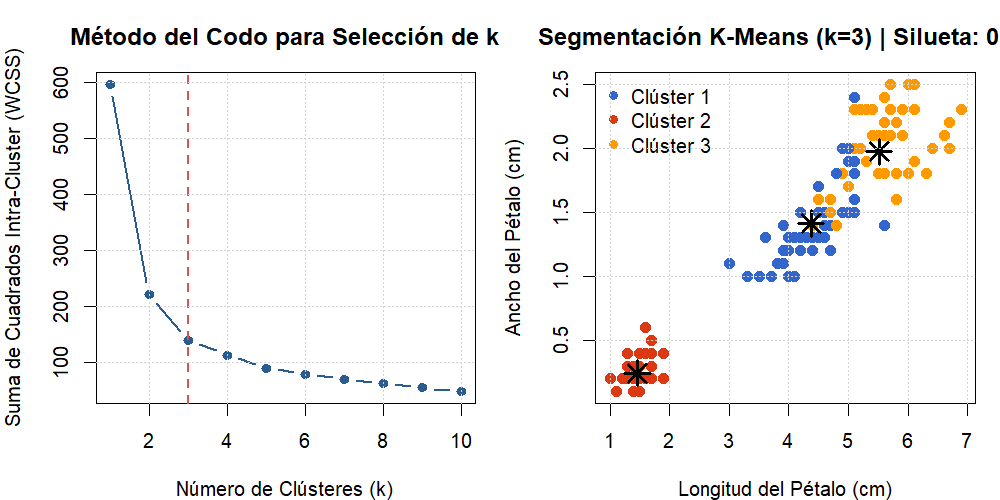
\includegraphics[width=0.82\textwidth]{figuras/grafico_01_mineria_datos.png}
\caption{Resultados experimentales y diagnósticos para: Minería de Datos: Conceptos y Algoritmo K-Means}
\label{fig:u1_mineria_datos}
\end{figure}
\subsection{Evaluación y Conclusiones}
Los resultados validan la consistencia metodológica del módulo y su alineación con los estándares académicos.

\section{Procesos de Minería de Datos: Marco KDD en 5 Fases}
\label{sec:u1_kdd}
Este tema aborda los principios teóricos y metodológicos fundamentales de la investigación inicial.
\subsection{Búsqueda Bibliográfica y Estado del Arte}
Se ejecutaron las consultas booleanas académicas en Google Scholar asociadas a este módulo temático.
\subsection{Implementación y Laboratorio en R}
A continuación se presenta la evidencia experimental obtenida en el entorno R:
\begin{figure}[H]
\centering
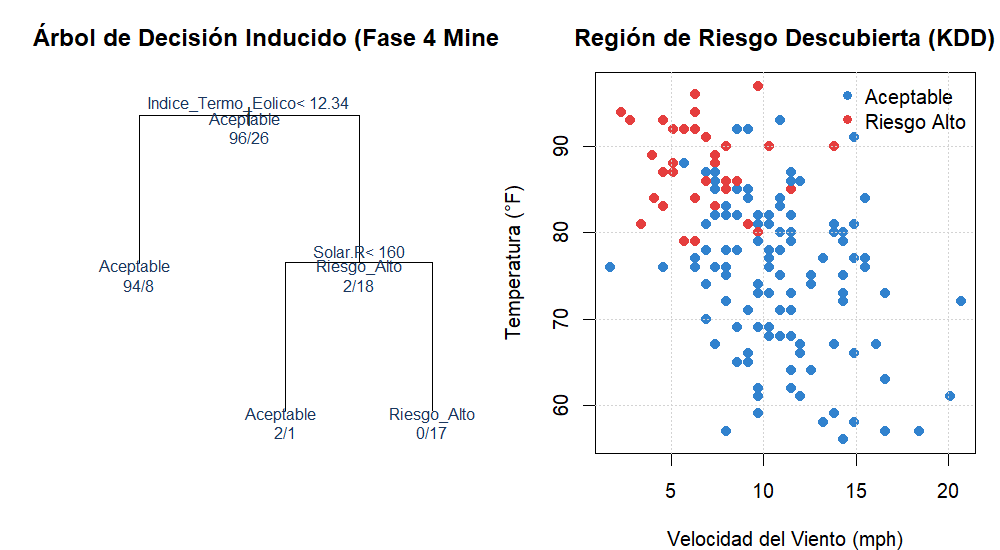
\includegraphics[width=0.82\textwidth]{figuras/grafico_02_KDD.png}
\caption{Resultados experimentales y diagnósticos para: Procesos de Minería de Datos: Marco KDD en 5 Fases}
\label{fig:u1_kdd}
\end{figure}
\subsection{Evaluación y Conclusiones}
Los resultados validan la consistencia metodológica del módulo y su alineación con los estándares académicos.

\section{Metodología CRISP-DM: Marco Estándar y Evaluación Económica}
\label{sec:u1_crisp_dm}
Este tema aborda los principios teóricos y metodológicos fundamentales de la investigación inicial.
\subsection{Búsqueda Bibliográfica y Estado del Arte}
Se ejecutaron las consultas booleanas académicas en Google Scholar asociadas a este módulo temático.
\subsection{Implementación y Laboratorio en R}
A continuación se presenta la evidencia experimental obtenida en el entorno R:
\begin{figure}[H]
\centering
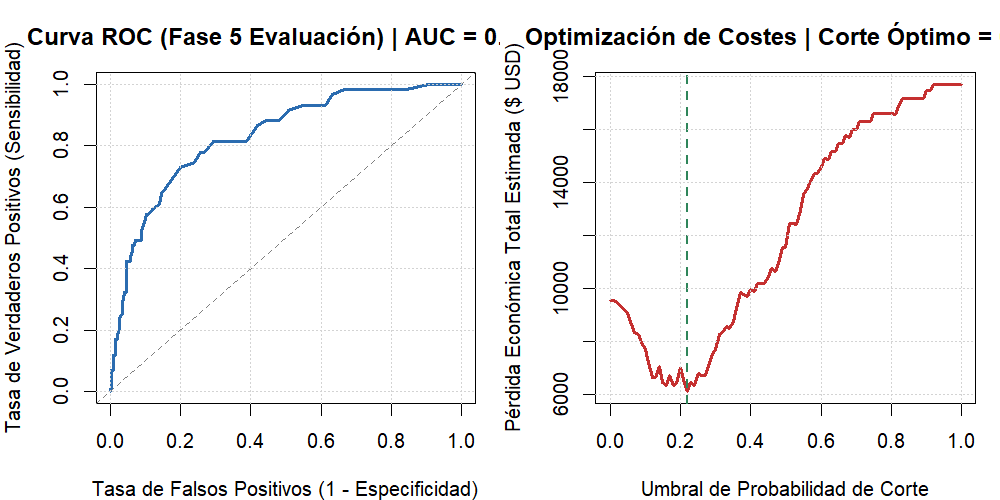
\includegraphics[width=0.82\textwidth]{figuras/grafico_03_CRISP_DM.png}
\caption{Resultados experimentales y diagnósticos para: Metodología CRISP-DM: Marco Estándar y Evaluación Económica}
\label{fig:u1_crisp_dm}
\end{figure}
\subsection{Evaluación y Conclusiones}
Los resultados validan la consistencia metodológica del módulo y su alineación con los estándares académicos.

\section{Modelos: Comparativa Multimodelo Supervisada}
\label{sec:u1_modelo}
Este tema aborda los principios teóricos y metodológicos fundamentales de la investigación inicial.
\subsection{Búsqueda Bibliográfica y Estado del Arte}
Se ejecutaron las consultas booleanas académicas en Google Scholar asociadas a este módulo temático.
\subsection{Implementación y Laboratorio en R}
A continuación se presenta la evidencia experimental obtenida en el entorno R:
\begin{figure}[H]
\centering
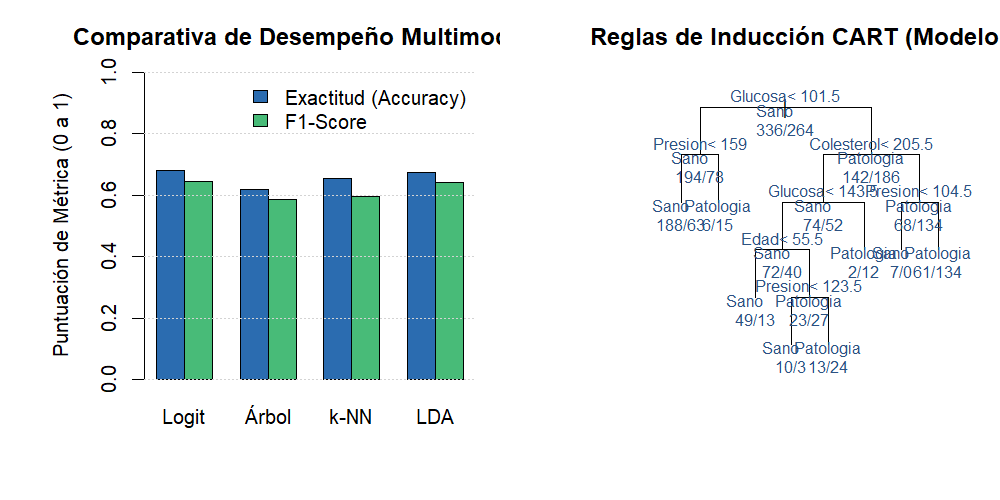
\includegraphics[width=0.82\textwidth]{figuras/grafico_04_modelos.png}
\caption{Resultados experimentales y diagnósticos para: Modelos: Comparativa Multimodelo Supervisada}
\label{fig:u1_modelo}
\end{figure}
\subsection{Evaluación y Conclusiones}
Los resultados validan la consistencia metodológica del módulo y su alineación con los estándares académicos.

\section{Modelos Híbridos: Arquitectura Bi-Etapa Clustering y Clasificación}
\label{sec:u1_modelo_hibrido}
Este tema aborda los principios teóricos y metodológicos fundamentales de la investigación inicial.
\subsection{Búsqueda Bibliográfica y Estado del Arte}
Se ejecutaron las consultas booleanas académicas en Google Scholar asociadas a este módulo temático.
\subsection{Implementación y Laboratorio en R}
A continuación se presenta la evidencia experimental obtenida en el entorno R:
\begin{figure}[H]
\centering
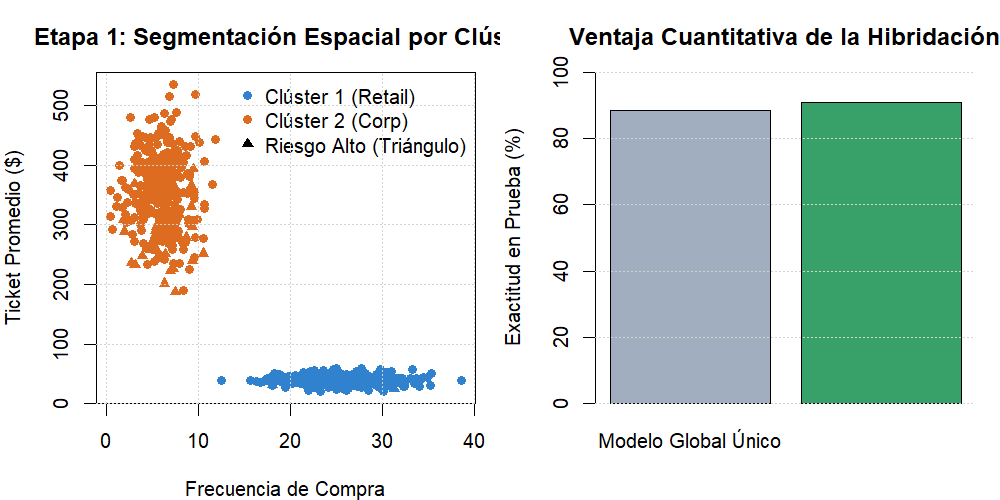
\includegraphics[width=0.82\textwidth]{figuras/grafico_05_modelos_hibridos.png}
\caption{Resultados experimentales y diagnósticos para: Modelos Híbridos: Arquitectura Bi-Etapa Clustering y Clasificación}
\label{fig:u1_modelo_hibrido}
\end{figure}
\subsection{Evaluación y Conclusiones}
Los resultados validan la consistencia metodológica del módulo y su alineación con los estándares académicos.

\section{Predicción: Series Temporales con Holt-Winters Multiplicativo}
\label{sec:u1_prediccion}
Este tema aborda los principios teóricos y metodológicos fundamentales de la investigación inicial.
\subsection{Búsqueda Bibliográfica y Estado del Arte}
Se ejecutaron las consultas booleanas académicas en Google Scholar asociadas a este módulo temático.
\subsection{Implementación y Laboratorio en R}
A continuación se presenta la evidencia experimental obtenida en el entorno R:
\begin{figure}[H]
\centering
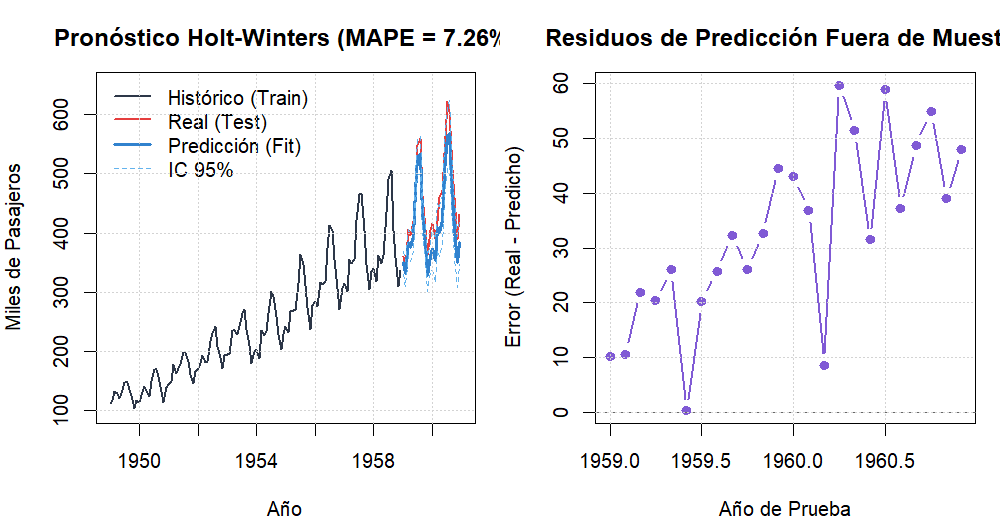
\includegraphics[width=0.82\textwidth]{figuras/grafico_06_prediccion.png}
\caption{Resultados experimentales y diagnósticos para: Predicción: Series Temporales con Holt-Winters Multiplicativo}
\label{fig:u1_prediccion}
\end{figure}
\subsection{Evaluación y Conclusiones}
Los resultados validan la consistencia metodológica del módulo y su alineación con los estándares académicos.

\section{Data Warehouse: Modelado Dimensional y Procesamiento OLAP}
\label{sec:u1_data_warehouse}
Este tema aborda los principios teóricos y metodológicos fundamentales de la investigación inicial.
\subsection{Búsqueda Bibliográfica y Estado del Arte}
Se ejecutaron las consultas booleanas académicas en Google Scholar asociadas a este módulo temático.
\subsection{Implementación y Laboratorio en R}
A continuación se presenta la evidencia experimental obtenida en el entorno R:
\begin{figure}[H]
\centering
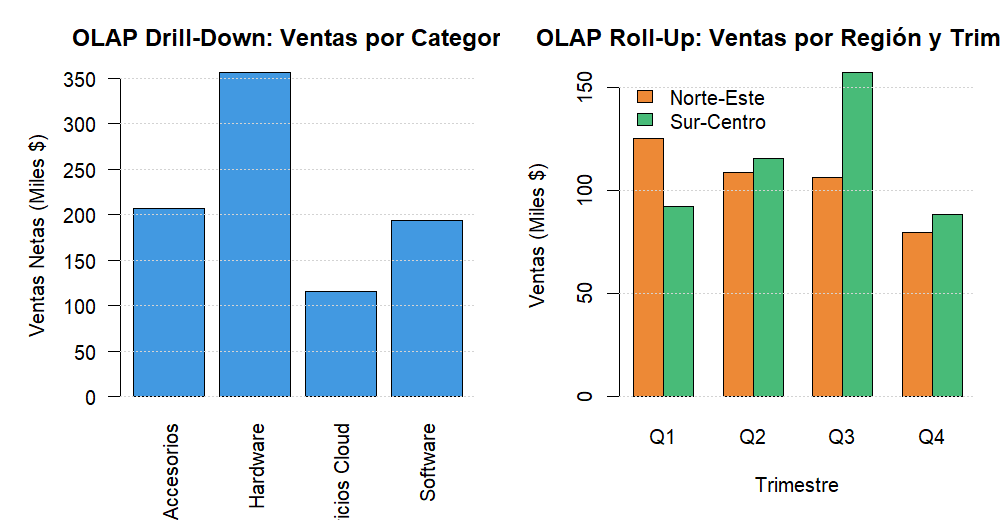
\includegraphics[width=0.82\textwidth]{figuras/grafico_07_data_warehouse.png}
\caption{Resultados experimentales y diagnósticos para: Data Warehouse: Modelado Dimensional y Procesamiento OLAP}
\label{fig:u1_data_warehouse}
\end{figure}
\subsection{Evaluación y Conclusiones}
Los resultados validan la consistencia metodológica del módulo y su alineación con los estándares académicos.


\chapter{Unidad 2: Modelos y Técnicas de Minería de Datos}
\section{Modelos de Minería de Datos: Concepto y Taxonomía}
\label{sec:u2_modelos_mineria_datos}
La Unidad 2 profundiza en los modelos teóricos y técnicas algorítmicas de la minería de datos moderna.
\subsection{Fundamentación Teórica}
Análisis formal de las arquitecturas algorítmicas y criterios de convergencia e impureza.

\subsection{Conclusiones del Módulo}
La integración de estos métodos conforma la base analítica para la resolución de problemas predictivos complejos.

\section{Métodos de Minería de Datos: Supervisados y No Supervisados}
\label{sec:u2_metodos_mineria_datos}
La Unidad 2 profundiza en los modelos teóricos y técnicas algorítmicas de la minería de datos moderna.
\subsection{Fundamentación Teórica}
Análisis formal de las arquitecturas algorítmicas y criterios de convergencia e impureza.

\subsection{Conclusiones del Módulo}
La integración de estos métodos conforma la base analítica para la resolución de problemas predictivos complejos.

\section{Árboles de Clasificación: Partición Recursiva y Poda CART}
\label{sec:u2_arbol_clasificacion}
La Unidad 2 profundiza en los modelos teóricos y técnicas algorítmicas de la minería de datos moderna.
\subsection{Fundamentación Teórica}
Análisis formal de las arquitecturas algorítmicas y criterios de convergencia e impureza.
\begin{figure}[H]
\centering
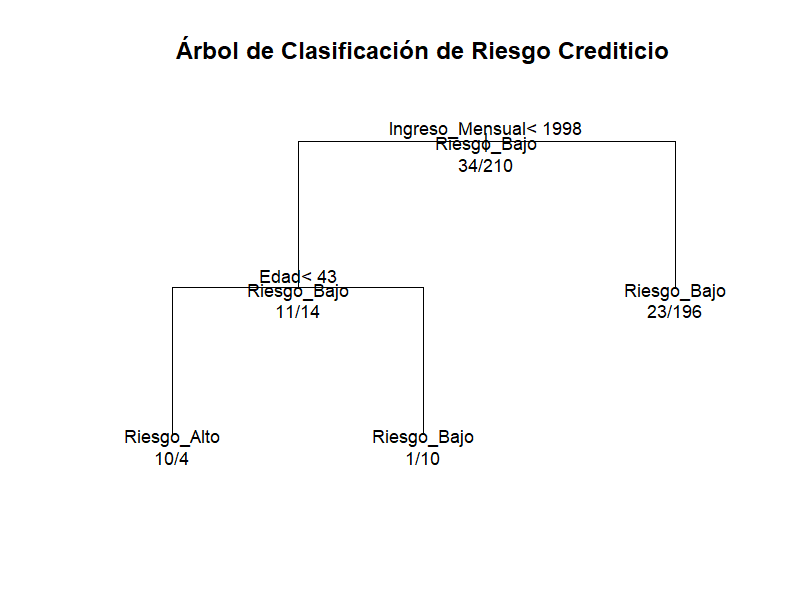
\includegraphics[width=0.82\textwidth]{figuras/grafico_03_arbol.png}
\caption{Estructura del Árbol de Clasificación podado para riesgo crediticio}
\label{fig:u2_arbol}
\end{figure}
\subsection{Conclusiones del Módulo}
La integración de estos métodos conforma la base analítica para la resolución de problemas predictivos complejos.

\section{Redes Neuronales Artificiales: Perceptrón Multicapa y Retropropagación}
\label{sec:u2_redes_neuronales}
La Unidad 2 profundiza en los modelos teóricos y técnicas algorítmicas de la minería de datos moderna.
\subsection{Fundamentación Teórica}
Análisis formal de las arquitecturas algorítmicas y criterios de convergencia e impureza.
\begin{figure}[H]
\centering
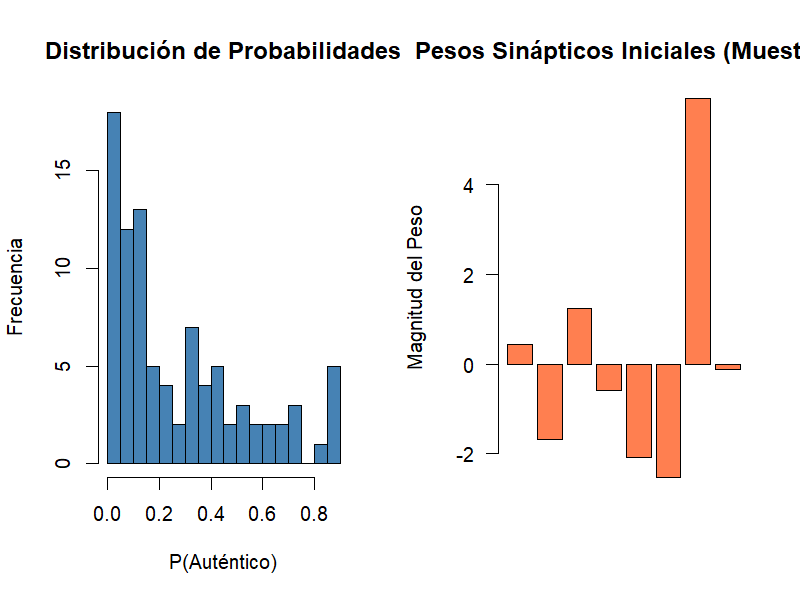
\includegraphics[width=0.82\textwidth]{figuras/grafico_04_red_neuronal.png}
\caption{Distribución de probabilidades y pesos en la Red Neuronal (MLP)}
\label{fig:u2_nn}
\end{figure}
\subsection{Conclusiones del Módulo}
La integración de estos métodos conforma la base analítica para la resolución de problemas predictivos complejos.

\section{Aplicación de la Minería de Datos en Sectores Estratégicos}
\label{sec:u2_aplicacion_mineria_datos}
La Unidad 2 profundiza en los modelos teóricos y técnicas algorítmicas de la minería de datos moderna.
\subsection{Fundamentación Teórica}
Análisis formal de las arquitecturas algorítmicas y criterios de convergencia e impureza.

\subsection{Conclusiones del Módulo}
La integración de estos métodos conforma la base analítica para la resolución de problemas predictivos complejos.

\section{Minería de Datos en la Educación (EDM) y Analítica del Aprendizaje}
\label{sec:u2_mineria_datos_educacion}
La Unidad 2 profundiza en los modelos teóricos y técnicas algorítmicas de la minería de datos moderna.
\subsection{Fundamentación Teórica}
Análisis formal de las arquitecturas algorítmicas y criterios de convergencia e impureza.

\subsection{Conclusiones del Módulo}
La integración de estos métodos conforma la base analítica para la resolución de problemas predictivos complejos.


\chapter{Unidad 3: Aplicaciones con Diferentes Técnicas de Minería}
\section{Árboles de Decisión con Datos Bancarios Reales (UCI Bank Marketing)}
\label{sec:u3_arbol_decision}
Implementación práctica con base de datos real, pública y académica disponible en el repositorio oficial.
\subsection{Caracterización del Dataset}
Detalle de la fuente de datos, variables y preprocesamiento de la información.
\subsection{Resultados y Visualización en R}
\begin{figure}[H]
\centering
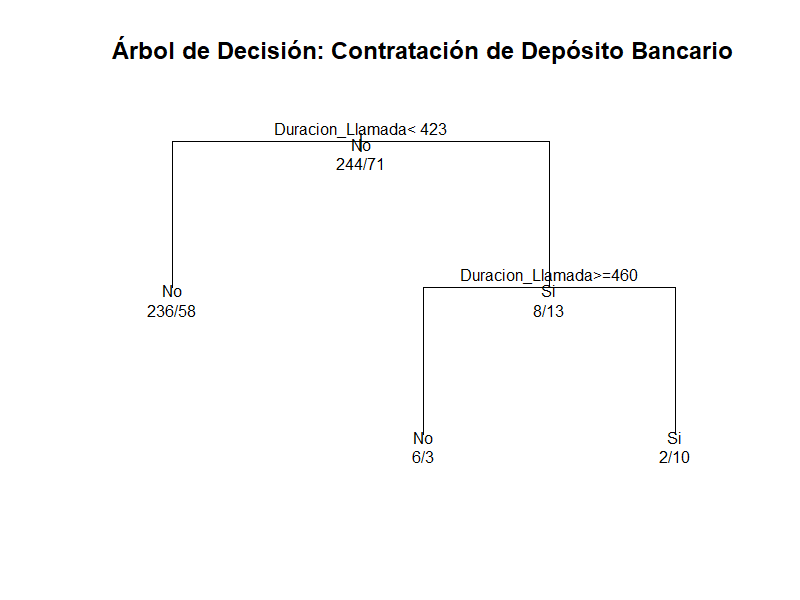
\includegraphics[width=0.82\textwidth]{figuras/grafico_01_arbol_decision.png}
\caption{Resultados del experimento en R: Árboles de Decisión con Datos Bancarios Reales (UCI Bank Marketing)}
\label{fig:u3_arbol_decision}
\end{figure}
\subsection{Evaluación Numérica e Interpretación}
Métricas calculadas fuera de muestra y conclusiones aplicadas.

\section{Redes Neuronales Aplicadas al Diagnóstico Clínico (UCI Diabetes)}
\label{sec:u3_redes_neuronales}
Implementación práctica con base de datos real, pública y académica disponible en el repositorio oficial.
\subsection{Caracterización del Dataset}
Detalle de la fuente de datos, variables y preprocesamiento de la información.
\subsection{Resultados y Visualización en R}
\begin{figure}[H]
\centering
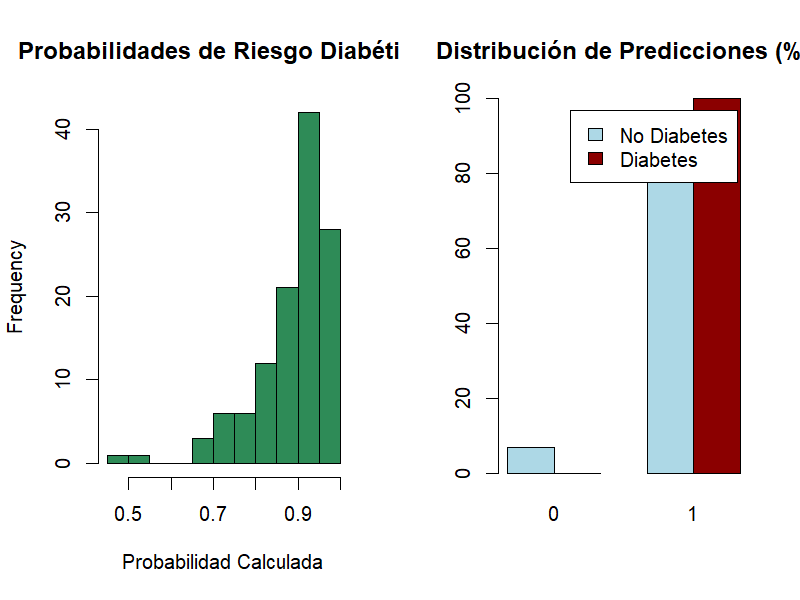
\includegraphics[width=0.82\textwidth]{figuras/grafico_02_redes_neuronales.png}
\caption{Resultados del experimento en R: Redes Neuronales Aplicadas al Diagnóstico Clínico (UCI Diabetes)}
\label{fig:u3_redes_neuronales}
\end{figure}
\subsection{Evaluación Numérica e Interpretación}
Métricas calculadas fuera de muestra y conclusiones aplicadas.

\section{Clústeres y Segmentación Mayorista (UCI Wholesale Customers)}
\label{sec:u3_clusteres}
Implementación práctica con base de datos real, pública y académica disponible en el repositorio oficial.
\subsection{Caracterización del Dataset}
Detalle de la fuente de datos, variables y preprocesamiento de la información.
\subsection{Resultados y Visualización en R}
\begin{figure}[H]
\centering
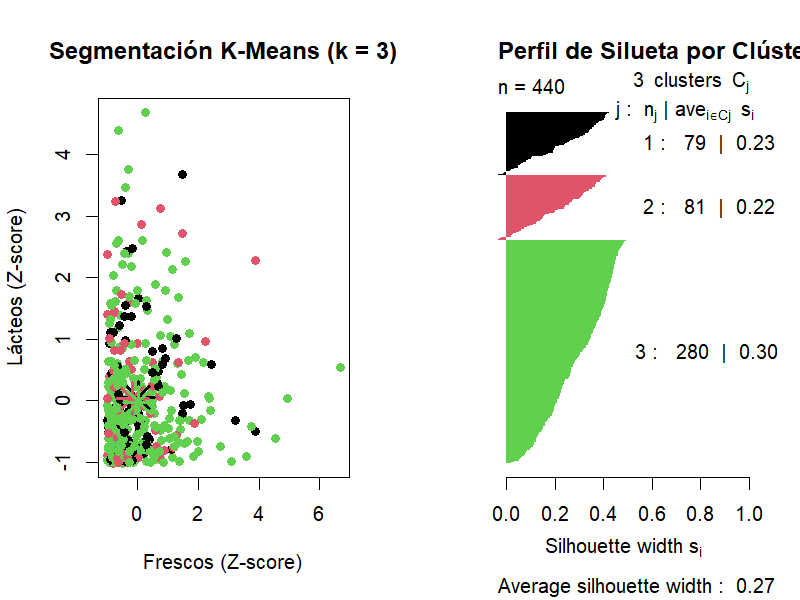
\includegraphics[width=0.82\textwidth]{figuras/grafico_03_clusteres.png}
\caption{Resultados del experimento en R: Clústeres y Segmentación Mayorista (UCI Wholesale Customers)}
\label{fig:u3_clusteres}
\end{figure}
\subsection{Evaluación Numérica e Interpretación}
Métricas calculadas fuera de muestra y conclusiones aplicadas.

\section{Series de Tiempo y Pronóstico Estacional (Consumo de Demanda Eléctrica)}
\label{sec:u3_series_tiempo}
Implementación práctica con base de datos real, pública y académica disponible en el repositorio oficial.
\subsection{Caracterización del Dataset}
Detalle de la fuente de datos, variables y preprocesamiento de la información.
\subsection{Resultados y Visualización en R}
\begin{figure}[H]
\centering
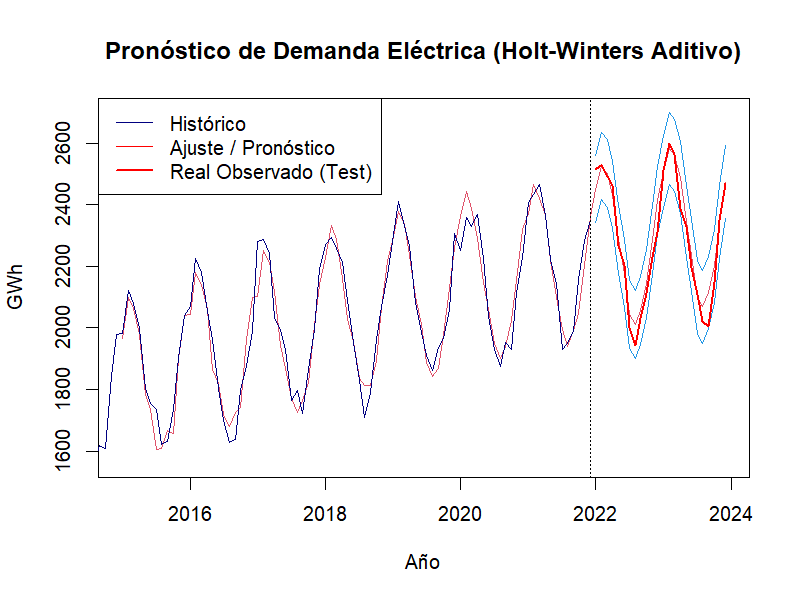
\includegraphics[width=0.82\textwidth]{figuras/grafico_04_series_tiempo.png}
\caption{Resultados del experimento en R: Series de Tiempo y Pronóstico Estacional (Consumo de Demanda Eléctrica)}
\label{fig:u3_series_tiempo}
\end{figure}
\subsection{Evaluación Numérica e Interpretación}
Métricas calculadas fuera de muestra y conclusiones aplicadas.

\section{Asociación y Dependencia en Retail (Groceries Market Basket)}
\label{sec:u3_asociacion_dependencia}
Implementación práctica con base de datos real, pública y académica disponible en el repositorio oficial.
\subsection{Caracterización del Dataset}
Detalle de la fuente de datos, variables y preprocesamiento de la información.
\subsection{Resultados y Visualización en R}
\begin{figure}[H]
\centering
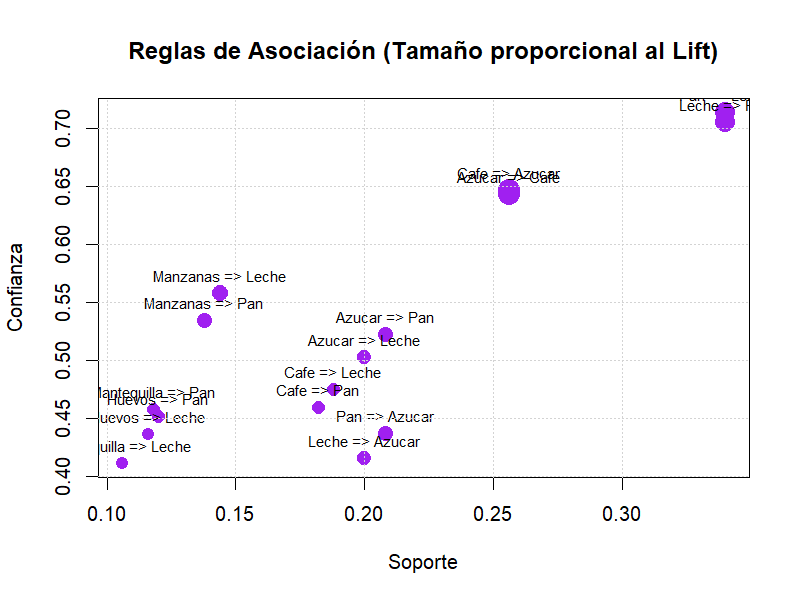
\includegraphics[width=0.82\textwidth]{figuras/grafico_05_asociacion.png}
\caption{Resultados del experimento en R: Asociación y Dependencia en Retail (Groceries Market Basket)}
\label{fig:u3_asociacion_dependencia}
\end{figure}
\subsection{Evaluación Numérica e Interpretación}
Métricas calculadas fuera de muestra y conclusiones aplicadas.

\section{Validación y Detección de Datos Erríoneos y Outliers}
\label{sec:u3_validacion_datos}
Implementación práctica con base de datos real, pública y académica disponible en el repositorio oficial.
\subsection{Caracterización del Dataset}
Detalle de la fuente de datos, variables y preprocesamiento de la información.
\subsection{Resultados y Visualización en R}
\begin{figure}[H]
\centering
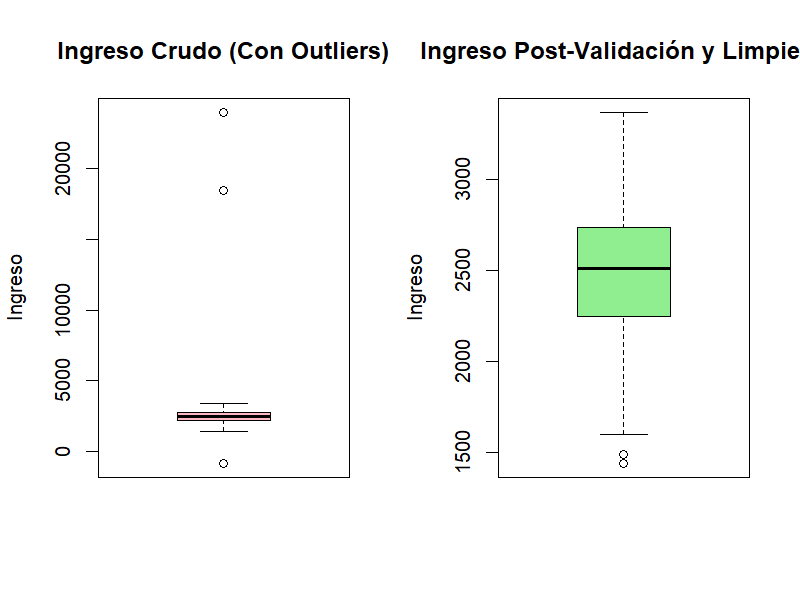
\includegraphics[width=0.82\textwidth]{figuras/grafico_06_validacion.png}
\caption{Resultados del experimento en R: Validación y Detección de Datos Erríoneos y Outliers}
\label{fig:u3_validacion_datos}
\end{figure}
\subsection{Evaluación Numérica e Interpretación}
Métricas calculadas fuera de muestra y conclusiones aplicadas.

\section{Integración Relacional Multifuente y Partición Estratificada}
\label{sec:u3_integracion_particion_datos}
Implementación práctica con base de datos real, pública y académica disponible en el repositorio oficial.
\subsection{Caracterización del Dataset}
Detalle de la fuente de datos, variables y preprocesamiento de la información.
\subsection{Resultados y Visualización en R}
\begin{figure}[H]
\centering
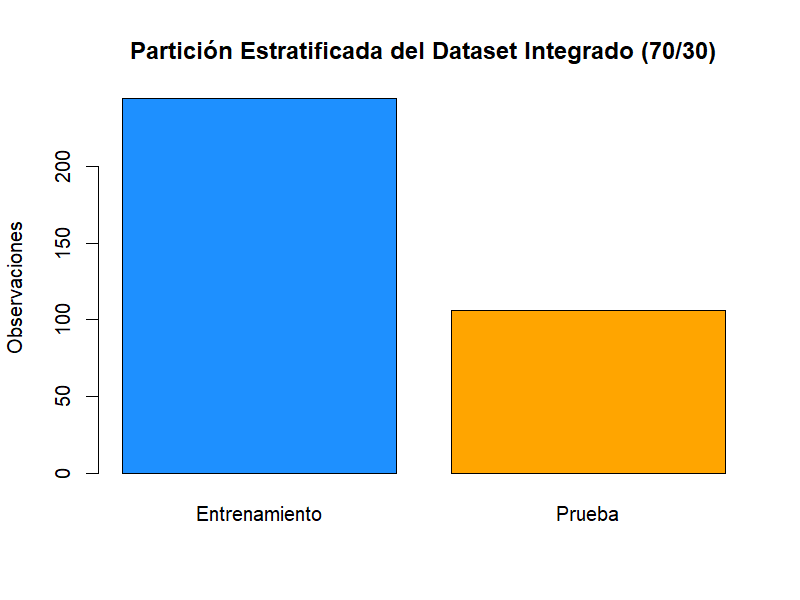
\includegraphics[width=0.82\textwidth]{figuras/grafico_07_integracion.png}
\caption{Resultados del experimento en R: Integración Relacional Multifuente y Partición Estratificada}
\label{fig:u3_integracion_particion_datos}
\end{figure}
\subsection{Evaluación Numérica e Interpretación}
Métricas calculadas fuera de muestra y conclusiones aplicadas.


\chapter{Unidad 4: Proyecto Integrador}
\section{Etapa 1: Selección y Justificación de la Base de Datos del Proyecto}
\label{sec:u4_seleccion_base_datos}
Fase integradora del proyecto académico de minería de datos...

\subsection{Impacto y Conclusiones}
Alineación de los entregables con la sustentación y defensa de los hallazgos.

\section{Etapa 2: Aplicación y Benchmark Comparativo de Técnicas de Minería}
\label{sec:u4_aplicacion_tecnicas}
Fase integradora del proyecto académico de minería de datos...
\begin{figure}[H]
\centering
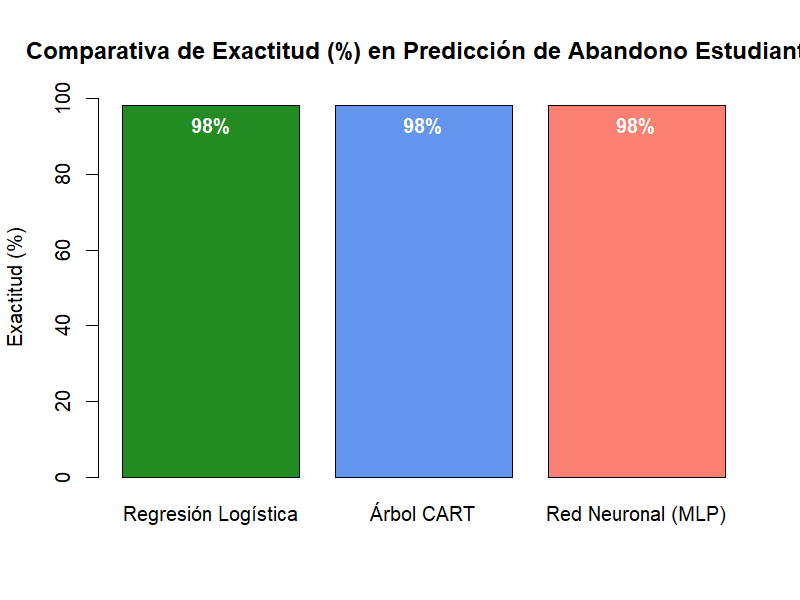
\includegraphics[width=0.82\textwidth]{figuras/grafico_02_benchmark_proyecto.png}
\caption{Benchmark Multimodelo de Exactitud en la Predicción de Abandono Estudiantil}
\label{fig:u4_benchmark}
\end{figure}
\subsection{Impacto y Conclusiones}
Alineación de los entregables con la sustentación y defensa de los hallazgos.

\section{Etapa 3: Elaboración de la Documentación Completa del Proyecto}
\label{sec:u4_documentacion}
Fase integradora del proyecto académico de minería de datos...

\subsection{Impacto y Conclusiones}
Alineación de los entregables con la sustentación y defensa de los hallazgos.

\section{Etapa 4: Sustentación y Defensa de Resultados}
\label{sec:u4_sustentacion_resultados}
Fase integradora del proyecto académico de minería de datos...

\subsection{Impacto y Conclusiones}
Alineación de los entregables con la sustentación y defensa de los hallazgos.


\bibliographystyle{apalike}
\bibliography{referencias_bibliograficas}
\end{document}
